\begin{center}
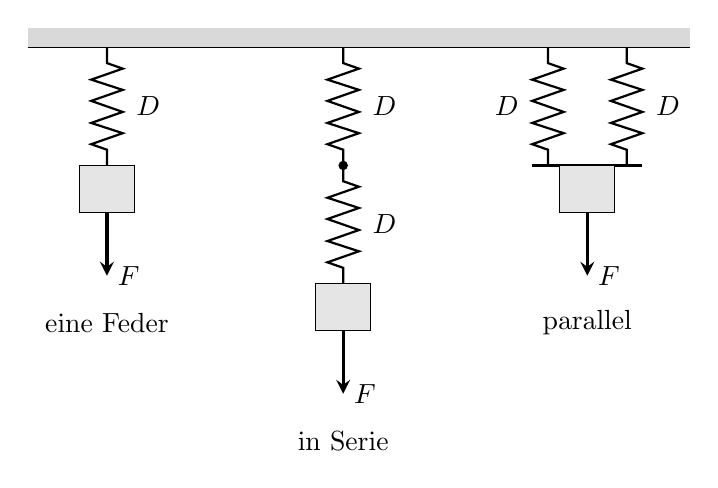
\begin{tikzpicture}[>=stealth]
 \fill[gray!30] (-1,0) rectangle (7.4,0.25);
 \draw (-1,0) -- (7.4,0);
 \draw[thick] (0.00,0.00) -- (0.00,-0.20) -- (0.20,-0.27) -- (-0.20,-0.41) -- (0.20,-0.54) -- (-0.20,-0.68) -- (0.20,-0.82) -- (-0.20,-0.96) -- (0.20,-1.09) -- (-0.20,-1.23) -- (0.00,-1.30) -- (0.00,-1.50);
 \node[right] at (0.25,-0.75) {$D$};
 \draw[fill=gray!20] (-0.35,-2.1) rectangle (0.35,-1.5);
 \draw[->, very thick] (0,-2.1) -- (0,-2.9) node[right] {$F$};
 \node at (0,-3.5) {eine Feder};
 \draw[thick] (3.00,0.00) -- (3.00,-0.20) -- (3.20,-0.27) -- (2.80,-0.41) -- (3.20,-0.54) -- (2.80,-0.68) -- (3.20,-0.82) -- (2.80,-0.96) -- (3.20,-1.09) -- (2.80,-1.23) -- (3.00,-1.30) -- (3.00,-1.50);
 \draw[thick] (3.00,-1.50) -- (3.00,-1.70) -- (3.20,-1.77) -- (2.80,-1.91) -- (3.20,-2.04) -- (2.80,-2.18) -- (3.20,-2.32) -- (2.80,-2.46) -- (3.20,-2.59) -- (2.80,-2.73) -- (3.00,-2.80) -- (3.00,-3.00);
 \fill (3,-1.5) circle (0.06);
 \node[right] at (3.25,-0.75) {$D$};
 \node[right] at (3.25,-2.25) {$D$};
 \draw[fill=gray!20] (2.65,-3.6) rectangle (3.35,-3.0);
 \draw[->, very thick] (3,-3.6) -- (3,-4.4) node[right] {$F$};
 \node at (3,-5.0) {in Serie};
 \draw[thick] (5.60,0.00) -- (5.60,-0.20) -- (5.80,-0.27) -- (5.40,-0.41) -- (5.80,-0.54) -- (5.40,-0.68) -- (5.80,-0.82) -- (5.40,-0.96) -- (5.80,-1.09) -- (5.40,-1.23) -- (5.60,-1.30) -- (5.60,-1.50);
 \draw[thick] (6.60,0.00) -- (6.60,-0.20) -- (6.80,-0.27) -- (6.40,-0.41) -- (6.80,-0.54) -- (6.40,-0.68) -- (6.80,-0.82) -- (6.40,-0.96) -- (6.80,-1.09) -- (6.40,-1.23) -- (6.60,-1.30) -- (6.60,-1.50);
 \node[left] at (5.35,-0.75) {$D$};
 \node[right] at (6.85,-0.75) {$D$};
 \draw[very thick] (5.4,-1.5) -- (6.8,-1.5);
 \draw[fill=gray!20] (5.75,-2.1) rectangle (6.45,-1.5);
 \draw[->, very thick] (6.1,-2.1) -- (6.1,-2.9) node[right] {$F$};
 \node at (6.1,-3.5) {parallel};
\end{tikzpicture}
\end{center}

An den Federn ziehe die Kraft $F$. Eine einzelne Feder dehnt sich dabei um $x = F/D$.

\emph{Aneinander gehängt (in Serie):} Jede der beiden Federn wird mit der ganzen Kraft $F$ gedehnt, also je um $F/D$. Die gesamte Verlängerung ist doppelt so gross:
\begin{align}
 x_\text{S} &= 2\cdot\frac{F}{D}
 \quad\Rightarrow\quad D_\text{S} = \frac{F}{x_\text{S}} = \result{\frac{D}{2}}
\end{align}

\emph{Nebeneinander (parallel):} Beide Federn werden gleich weit gedehnt und teilen sich die Kraft, jede trägt $F/2$:
\begin{align}
 x_\text{P} &= \frac{F/2}{D} = \frac{F}{2D}
 \quad\Rightarrow\quad D_\text{P} = \frac{F}{x_\text{P}} = \result{2D}
\end{align}
